\section{Index Compression}\label{ch6}
In this chapter, we employ a number of compression techniques for dictionary and inverted index that are essential for efficient IR systems.

There are two more subtle \textbf{benefits} of compression:

\begin{enumerate}
    \item Increased use of \textbf{caching}: with compression, we can fit a lot more information into main memory. Instead of having to expend a disk seek when processing a query, we instead access its postings list in memory and decompress it. As we will see below, there are simple and efficient decompression methods, so that the penalty of having to decompress the postings list is small. As a result, we are able to \textbf{decrease the response time} of the IR system substantially;
    \item \textbf{Faster transfer of data from disk to memory}. Efficient decompression algorithms run so fast on modern hardware that the total time of transferring a compressed chunk of data from disk and then decompressing it is usually less than transferring the same chunk of data in uncompressed form.
\end{enumerate}

However, if the goal of compression is to conserve disk space and to decrease the response time of the IR system, then the \textbf{speed of the compression algorithm} itself is crucial: the compression algorithms we discuss in this chapter are highly efficient and can therefore serve all the purposes of index compression.

\underline{NOTE}: in this Chapter, we define a \textit{posting} as a docID in a postings list. For example, (6; 20, 45, 100), where 6 is the termID of the list's term, contains three postings.

\subsection{Statistical properties of terms in IR}
As in Chapter \ref{ch5}, we use \textit{Reuters-RCV1} as our model collection. We recall it main statistics in Picture \ref{reuters}, while in Picture \ref{statistics} we provide some terms and postings statistics of the collection.

\begin{figure}[h!]
		\centering
		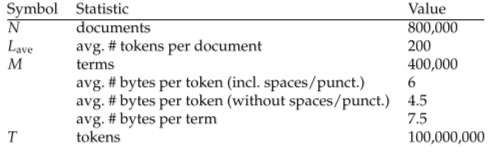
\includegraphics[scale = 1.5]{img/reuters.jpg}
		\label{reuters}
        \caption{Main statistics of \textit{Reuters-RCV1} collection}
\end{figure}

\begin{figure}[h!]
		\centering
		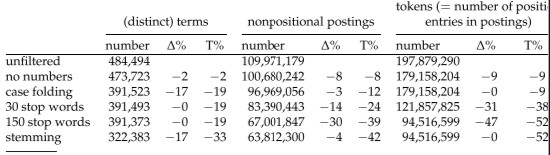
\includegraphics[scale = 1.7]{img/statistics.jpg}
		\label{statistics}
        \caption{Terms and postings statistics of \textit{Reuters-RCV1} collection}
\end{figure}

Some notes about these statistics follow:

\begin{itemize}
    \item the "$\Delta \%$" represents the reduction in size from the previous line;
    \item the "T\%" is the cumulative reduction from unfiltered;
    \item in general, the statistics show that \textbf{pre-processing} affects the size of the \textbf{dictionary} and the number of \textbf{non-positional postings} greatly: as we can see, stemming and case folding (i.e. considering "Rome" and "rome" as the same term) reduce the number of distinct terms by 17\%;
    \item the treatment of stopwords is also important: eliminating the 30 and 150 most common words from indexing cuts 31\% and 47\% of the total number of entries in postings, and 14\% and 30\% of the non-positonal postings;
    \item however, we notice that the usage of case folding and stemming does not change the number of entries in postings: this happens beacuse the positions of the terms are still kept in the postings;
    \item the same thing happens with the stopwords w.r.t. the number of distinct terms: we're only cutting off 30/150 words over a total of half million terms!
\end{itemize}

The compression techniques we describe in the remainder of this chapter are \textbf{lossless}, that is, \textbf{all information is preserved}. Better compression ratios can be achieved with \textbf{lossy} compression, which discards some information. Case folding, stemming, and stop word elimination are forms of lossy compression. In general, lossy compression makes sense when the “lost” information is unlikely ever to be used by the search system. For example, web search is characterized by a large number of documents, short queries, and users who only look at the first few pages of results. As a consequence, we can discard postings of documents that would only be used for hits far down the list. Thus, there are retrieval scenarios where lossy methods can be used for compression without any reduction in effectiveness.

Before introducing techniques for compressing the dictionary, we want to estimate the \textbf{number of distinct terms} (size of the vocabulary) $M$ in a collection. First of all, we notice that we cannot assume an upper bound; in practice, we will discover that the vocabulary size keep growing with the collection size.

\subsubsection{Heap's Law: estimating the number of terms}
The \textbf{Heap's Law} estimates the vocabulary size as a function of the collection size, in particular:

$$
M = kT^b
$$

, where:

\begin{itemize}
    \item $T$ is the number of tokens in the collection;
    \item $30 \leq k \leq 100$;
    \item $b \sim 0.5$.
\end{itemize}

The motivation of this law resides in the \textbf{linear relationship} between the collection size and the vocabulary size in a \textbf{log-log plot}, as represented in Picture \ref{heap}. 

\begin{figure}[h!]
		\centering
		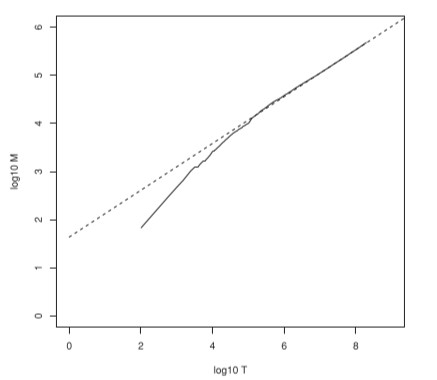
\includegraphics[scale = 1.7]{img/Heap law.jpg}
		\label{heap}
        \caption{Heap's Law: linear relationship between $M$ and $T$ in a log-log scale}
\end{figure}

As we can see, for RCV1 collection, the dashed line $\log_{10}M = 0.49 * \log_{10} T + 1.64$ represents the best least-square fit: in this case, $b = 0.49$ and $k = 44$. For example, for the first 1,000,020 tokens, Heap's Law predicts $44 * 1,000,020^{0.49} = 30,323$ terms, while the dashed line predicts 38,365 terms, so it is a good approximation.

Notice that the parameter $k$ is quite variable because vocabulary growth depends a lot on the nature of the collection and how it is processed. Case-folding and stemming reduce the growth rate of the vocabulary, whereas including numbers and spelling errors increase it.

In general, regardless of the values of the parameters for a particular collection, Heaps’ law suggests that:

\begin{enumerate}
    \item The dictionary size continues to increase with more documents in the collection, rather than a maximum vocabulary size being reached;
    \item The size of the dictionary is quite large for large collections
\end{enumerate}

These two hypotheses have been empirically shown to be true of large text collections, so dictionary compression is a crucial operation for an effective IR system.

\underline{Exercise}: Compute the vocabulary size for this scenario. There are 3,000 different terms ($M_1$) in the first 10,000 tokens ($T_1$), and 30,000 different terms ($M_2$) in the first 1,000,000 tokens($T_2$). Assume a search engine indexes a total of 20,000,000,000 (= $2^{10}$) pages, each containing 200 tokens on average. What is the size of the vocabulary of the indexed collection as predicted by the Heap's Law? 

\subsubsection{Zipf's Law}
While Heap's Law gives the vocabulary size, \textbf{Zipf's Law} helps us understanding how the terms are distributed across documents, so it takes into account the relative frequencies of terms, as we know that in natural languages, there are a few very frequent terms and very many rare terms.

If we assume that the terms are ranked from the most frequent to the least frequent, we can consider:
\begin{itemize}
    \item $t_i$ to be the term at rank $i$ in the collection;
    \item $cf_i$ to be the collection frequency, i.e. the number of occurrences of the term $t_i$, i.e. the term at rank $i$, in the collection;
    \item $df_i$ to be the document frequency, i.e. the total number of documents that contain the term $t_i$ in the corpus;
    \item $tf_{i,d}$ to be the term frequency, i.e. the total number of occurrences of the term in a document
\end{itemize}

Zipf's Law states that if $t_1$ is the most common term in the collection, $t_2$ is the next most common, and so on, then the collection frequency $cf_i$ of the i-th
most common term is proportional to $1/i$, i.e.:

$$
cf_i \propto \frac{1}{i}
$$

In this sense, if the most frequent term occurs $cf_i$ times, then the second most common will occur half of the occurrences, and the third one third of the occurrences and so on.. Another way of stating Zipf's Law is:

$$
cf_i = ci^{-1}
$$

or

$$
\log cf_i = \log c  - \log i
$$

, where $c$ is a constant. As we can see, there is a linear relationship between $\log cf_i$ and $\log i$, with slope -1, as represented in Picture \ref{zip}.

\begin{figure}[h!]
		\centering
		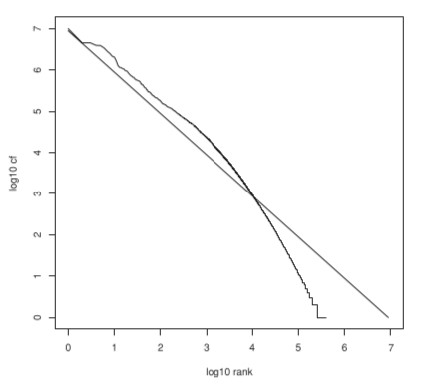
\includegraphics[scale = 1.7]{img/zipf law.jpg}
		\label{zip}
        \caption{Zipf's Law: linear relationship between $cf_i$ and $i$ in a log-log scale}
\end{figure}

Moreover, if we consider the relationship $cf_i = ci^{-1}$, we can recognize a \textbf{Power Law relationship}: the Power Law states that $p(i) \approx k i^{-\alpha}$, i.e. that roughly 80\% of the total popularity comes from 20\% of the terms. Notice that the quantity $\alpha$ represents the slope in the log-log plot of $p$ and $i$.

\subsection{Dictionary compression}
This section presents a series of dictionary data structures that achieve increasingly higher compression ratios. The main reason for compressing the dictionary is to fit it in memory, in order to reduce the number of disk accesses when processing a query. Indeed, some embedded/small devices may have very little memory. 

\subsubsection{Dictionary as a string}
The simplest data structure for the dictionary is to sort the vocabulary lexicographically and store it in an \textbf{array of fixed-width entries} as shown in Picture \ref{dic string}.

\begin{figure}[h!]
		\centering
		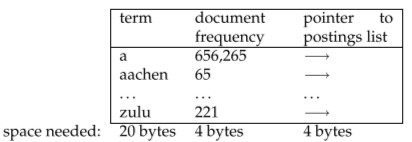
\includegraphics[scale = 1.7]{img/dictionary string.jpg}
		\label{dic string}
        \caption{Dictionary as an array of fixed-width entries}
\end{figure}

If we allocate 20 bytes for the term itself, 4 bytes for its document frequency and 4 bytes for its pointer to its postings list, then for Reuters-RCV1 we need 400,000 x 28 = 11.2 MB for storing the dictionary. Notice that the lexicographical order allows us to perform a binary search for looking up terms. However, using fixed-width entries for terms is clearly wasteful, since the average length of a term in English is about eight characters, so on average we are wasting twelve characters. Also, we have no way of storing terms with more than twenty characters. 

We can overcome these issues by storing the dictionary terms as one \textbf{long string of characters}, as shown in Picture \ref{dic string 2}.

\begin{figure}[h!]
		\centering
		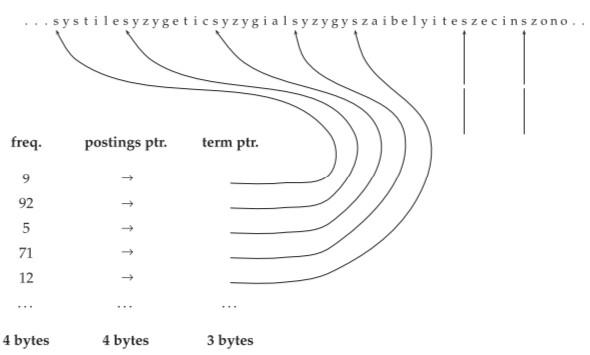
\includegraphics[scale = 1.7]{img/dictionary string_2.jpg}
		\label{dic string 2}
        \caption{Dictionary as a string}
\end{figure}

In this case, for each term we use 4 bytes for storing the term frequency, 4 bytes for storing the pointer to the corresponding postings list, 3 bytes for storing the term pointer and an average of 8 bytes for storing the term in the string. In this way, we only use an average of 11 bytes per term, versus the 20 bytes we used before, resulting in a 60\% storage save. In this case, we have a total of 19 bytes, so 400,000 x 19 = 7.6 MB, against the 11.2 MB used in the fixed-width entries. Notice that, as before, the look for a term can be done by performing a binary search operation, and that in this case the end of the string is not stored, since the term pointer of the next term is used as indicator of the end of the current term.

\subsubsection{Blocked storage}
We can further compress the dictionary by grouping terms in the string into blocks of size $k$ and keeping a term pointer only for the first term of each block, as represented in Picture \ref{blocked}.

\begin{figure}[h!]
		\centering
		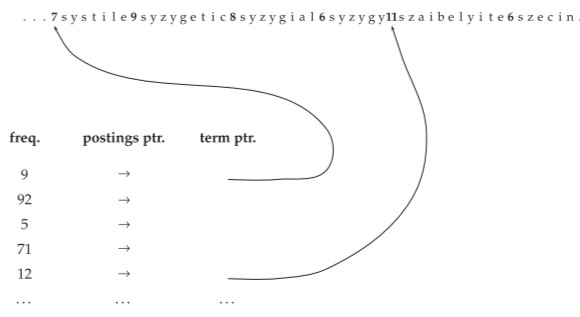
\includegraphics[scale = 1.7]{img/blocked storage.jpg}
		\label{blocked}
        \caption{Blocked storage}
\end{figure}

In this case we store the length of the term in the string as an additional byte at the beginning of the term: we thus eliminate $(k-1)$ term pointers, but need an additional $k$ bytes for storing the length of each term. If $k = 4$ we save $(k-1)$ x 3 = 9 bytes for term pointers, but we need an additional $k = 4$ bytes for term lengths. In the case of Reuters-RCV1, we reduce 5 bytes per four-term block, resulting in a total of 0.5 MB, bringing us down to 7.1 MB.

By increasing the block size k, we get better compression. However, there is a \textbf{tradeoff} between \textbf{compression} and the \textbf{speed of term lookup}. Suppose we have an eight-term dictionary, as represented in Picture \ref{example}.

\begin{figure}[h!]
		\centering
		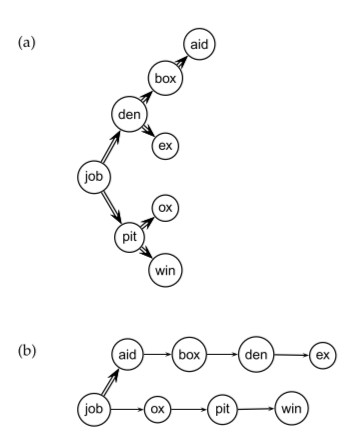
\includegraphics[scale = 1.7]{img/example .jpg}
		\label{example}
        % \caption{Search on uncompressed and compressed dictionary}
\end{figure}

In the Picture, steps in binary search are showed as double lines, and steps in list search as simple lines. We search for terms in the uncompressed dictionary by binary search (a). In the compressed dictionary, we first locate the term’s block by binary search and then its position within the list by linear search through the block (b). Searching the uncompressed dictionary in (a) takes on average (0 + 1 + 2 + 3 + 2 + 1 + 2 + 2)/8, i.e. more or less 1.6 steps, assuming each term is equally likely to come up in a query. For example, finding the two terms, \textit{aid} and \textit{box}, takes three and two steps, respectively. With blocks of size k = 4 in (b), we need (0+1+2+3+4+1+2+3)/8 = 2 steps on average, i.e. 25\% more. By increasing k, we can get the size of the compressed dictionary arbitrarily close to the minimum of 400,000 × (4 + 4 + 1 + 8) = 6.8 MB, but term lookup becomes prohibitively slow for large values of k.

However, by now we did not exploit the redundancy in the dictionary, in particular the fact that consecutive entries in an alphabetically sorted list share common prefixes. The exploitation of this property leads to \textit{front coding}.

\begin{figure}[h!]
		\centering
		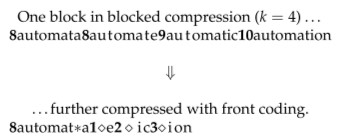
\includegraphics[scale = 2.0]{img/front coding.jpg}
		\label{front}
        \caption{Front coding: first implementation}
\end{figure}

In this case, a \textbf{common prefix} is identified for a sub-sequence of the term list, and then referred to with a special character. As we can see, the compression with front coding includes the common prefix, and each of the following characters for each term in the uncompressed sub-sequence. Together with the characters, the extra length beyond the suffix is stored, leading to a much smaller representation. In the case of Reuters-RCV1, this strategy saves another 1.2 MB. However, this is not the only possible implementation of the idea of front coding: Picture \ref{front2} show another implementation in which each term exploits a prefix of the previous one.

\begin{figure}[h!]
		\centering
		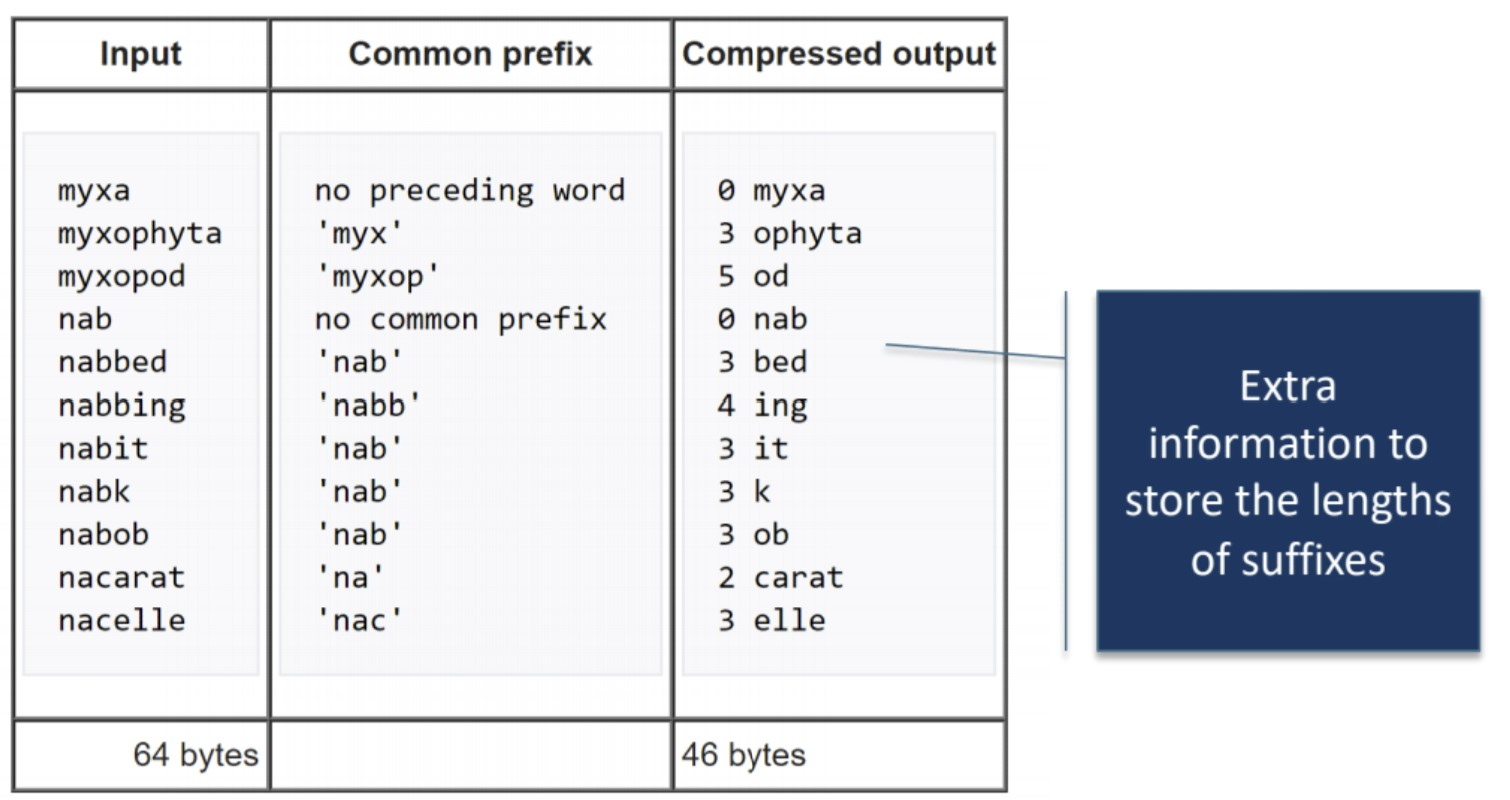
\includegraphics[scale = 0.5]{img/front coding2.jpg}
		\label{front2}
        \caption{Front coding: second implementation}
\end{figure}

However, even with the best compression scheme, it may not be feasible to store the entire dictionary in main memory for very large text collections and for hardware with limited memory. Picture \ref{summary} provides a summary of the dictionary compression achieved using the data structures we described so far.

\begin{figure}[h!]
		\centering
		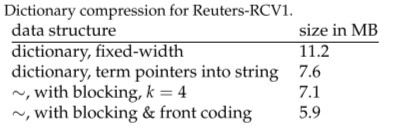
\includegraphics[scale = 2.0]{img/summary compression.jpg}
		\label{summary}
        \caption{Dictionary compression: summary}
\end{figure}

\subsection{Postings compression}
We recall the statistics of Reuters-RCV1 collection: as we can see, the number of postings, i.e. the number of docIDs in a postings list, is 100,000,000. DocIDs are $\log_{2}800,000 \approx 20$ bits long, so the size of the collection is 800,00 x 200 x 6 bytes = 960 MB, while the size of the uncompressed postings file is 100,000,000 x 20/8 = 150 MB.

\begin{figure}[h!]
		\centering
		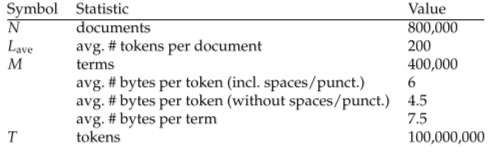
\includegraphics[scale = 1.5]{img/reuters.jpg}
		\label{reuters}
        \caption{Main statistics of \textit{Reuters-RCV1} collection}
\end{figure}

To use a more efficient representation of the postings file, i.e. a representation that uses less than 20 bits per document, we can exploit the fact that postings for frequent terms are close together. As represented in Picture \ref{gaps}, a very \textbf{frequent term} will have postings whose \textbf{gaps} are very \textbf{close}, and for which much less than 20 bits can be used, so in this case the idea is to store the gaps instead of the docIDs; on the other hand, gaps for a \textbf{rare term} have the \textbf{same order of magnitude as the docIDs}, so they need 20 bits. In this sense, we need a \textit{variable encoding} method that uses fewer bits for smaller gaps.

\begin{figure}[h!]
		\centering
		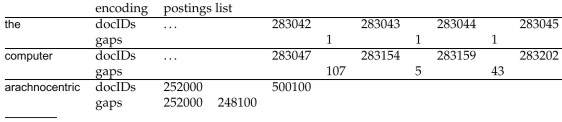
\includegraphics[scale = 2.0]{img/gaps.jpg}
		\label{gaps}
        \caption{Encoding gaps}
\end{figure}

To encode small numbers in less space than large numbers, we look at two types of methods: \textbf{bytewise compression} and \textbf{bitwise compression}. As the names suggest, these methods attempt to encode gaps with the minimum number of bytes and bits, respectively.

\subsubsection{Variable byte encoding}
Variable byte (VB) encoding uses an integral number of bytes to encode a gap $G$:

\begin{itemize}
    \item the last 7 bits of a byte are \textit{payload} and encode part of the gap;
    \item the first bit of the byte is a \textit{continuation bit}: it is set to 1 for the last byte of the encoded gap and to 0 otherwise.
\end{itemize}

To decode a variable byte code, we read a sequence of bytes with continuation bit 0 terminated by a byte with continuation bit 1. We then extract and concatenate the 7-bit parts. An example of VB-encoded postings list is provided in Picture \ref{vb}.

\begin{figure}[h!]
		\centering
		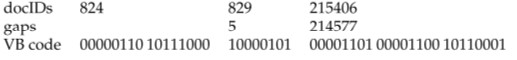
\includegraphics[scale = 2.0]{img/VB encoding.jpg}
		\label{vb}
        \caption{Example of VB encoding}
\end{figure}

A key property of VB encoding is that VB-encoded postings are \textbf{uniquely prefix-decodable}, i.e. no whole code word in the system is a prefix of any other code word. This means that no special marker is needed to separate codes.

With VB compression, the size of the compressed index for Reuters-RCV1 is 116 MB as we verified in an experiment: this is a more than 50\% reduction of the size of the uncompressed index. 

The idea of VB encoding can also be applied to larger or smaller units than bytes: 32-bit words, 16-bit words, and 4-bit words or nibbles. \textbf{Larger words} further \textbf{decrease} the \textbf{amount of bit manipulation} necessary at the cost of less effective (or no) compression. In general, \textbf{bytes} offer a \textbf{good compromise} between \textbf{compression ratio} and \textbf{speed of decompression}, and for most IR systems \textbf{variable byte codes} offer an excellent \textbf{tradeoff} between \textbf{time} and \textbf{space}, and they are also simple to implement. However, if the disk space is a scarce resource, we can achieve better compression ratios by using bit-level encodings, in particular two closely related encodings: $\gamma$ codes, which we will turn to next, and $\delta$ codes.

\subsubsection{Elias-$\gamma$ encoding}
While VB codes use a variable number of bytes for encoding a gap, bit-level codes use a finer grained bit level. The simplest bit-level code is the \textbf{unary code}, which represents $n$ as a string of $n$ 1's followed by a 0, as showed in the first column of Picture \ref{gamma}.

\begin{figure}[h!]
		\centering
		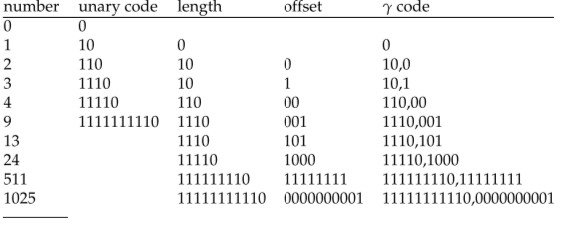
\includegraphics[scale = 2.0]{img/gamma encoding.jpg}
		\label{gamma}
        \caption{Examples of unary and $\gamma$ codes}
\end{figure}

Clearly, the unary code is not efficient, but it will become handy later.

In general, how efficient can a code be in principle? Assuming the $2^n$ gaps $G$ with $1 \leq G \leq 2^n$ are all equally likely, the optimal encoding uses $n$ bits for each $G$. So some gaps cannot be encoded with fewer than $\log_2 G$ bits. Our goal is to get as close to this lower bound as possible.

A method that is within a factor of optimal is $\gamma$ encoding. $\gamma$ codes implement \textbf{variable-length encoding} by \textbf{splitting} the representation of a gap $G$ into a pair of \textbf{length} and \textbf{offset}:

\begin{itemize}
    \item the \textit{offset} is $G$ in binary, but with the leading 1 removed. For example, for 13 (binary 1101), the \textit{offset} is 101;
    \item the \textit{length} encodes the length of \textit{offset} in unary code. For 13, the length of \textit{offset} is 3 bits, which is 1110 in unary.
\end{itemize}

The $\gamma$ code is then the \textbf{concatenation} of \textit{length} and \textit{offset} (in the example, the $\gamma$ code of 13 is therefore 1110101). Picture \ref{gamma} provides some other examples. The \textbf{encoding} of a $\gamma$ code works as follows:

\begin{enumerate}
    \item Read the unary code up to the 0 that terminates it, for example the four bits 1110 when decoding 1110101. Now we know that the offset is long 3 bits;
    \item The offset is read correctly, and the 1 is preprended, leading to 1101 = 13.
\end{enumerate}

In general:

\begin{itemize}
    \item the length of the \textit{offset} is $\lfloor \log_2 G \rfloor$ bits;
    \item the length of the \textit{length} is $\lfloor \log_2 G \rfloor + 1$
\end{itemize}

so the length of the entire code is $2 \lfloor \log_2 G \rfloor + 1$ bits. 

All the $\gamma$ codes have an odd number of bits, and they are within a factor of 2 of the optimal encoding $\log_2 G$ for any distribution, which makes the $\gamma$ codes to be \textbf{universal}. In addition to universality, $\gamma$ codes are \textbf{prefix free}, i.e. no $\gamma$ code can be the prefix of another, meaning that there is always a unique decoding of a sequence of $\gamma$ codes. The other property is that $\gamma$ codes are \textbf{parameter free}, which simplifies the implementation and the decompression of this code. However, a \textbf{disadvantage} of this encoding is that it is relatively inefficient for large numbers, since the unary code is used for encoding the offset.

The result of running $\gamma$ compression on Reuters-RCV1 is that the size of the compressed index is 101 MB, which is less than VB encoding.

Picture \ref{summary with post} shows a summary of the results of the compression techniques we exploited thus far.

\begin{figure}[h!]
		\centering
		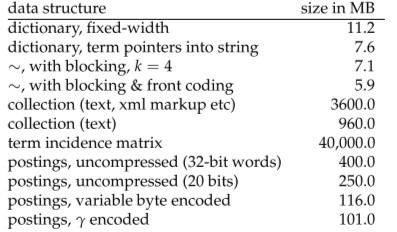
\includegraphics[scale = 2.0]{img/summary with postings.jpg}
		\label{summary with post}
        \caption{Summary of compression techniques including postings}
\end{figure}

\subsubsection{Elias-$\delta$ encoding}
A slight variation of the $\gamma$ codes are the $\delta$, in which again the gap $G$ is represented into a pair of \textit{length} and \textit{offset}:

\begin{itemize}
    \item the \textit{offset} is $G$ in binary, but with the leading 1 removed. For example, for 13 (binary 1101), the \textit{offset} is 101. It is the same as $\gamma$ codes;
    \item the \textit{length} encodes the length of \textit{offset} in $\gamma$ code.
\end{itemize}

In this case, $\delta$ encoding uses $2 \lfloor \log_2 \lfloor \log_2 G \rfloor \rfloor + 1$ bits.

\subsubsection{Golomb-Rice encoding}
Golomb-Rice encoding works as follows: we choose a quantity $M = 2^j$, where $j$ is a parameter of the method, and we encode an integer $n$ by splitting $n$ into two components, the quotient $q(n)$ and the remainder $r(n)$, where:

\begin{itemize}
    \item $q(n) = \lfloor \frac{n-1}{M} \rfloor$;
    \item $r(n) = (n-1) mod M$, i.e. $0 \leq r(n) \leq M - 1$.
\end{itemize}

Then, $n$ is encoded by writing $q(n) + 1$ in unary, followed by $r(n)$ as a binary number represented on $\log_2 M$ (= $j$) bits. In general, $j$ is chosen so that $2^j$ is centered around the mean of the elements to be represented.

\subsubsection{Interpolative coding}
A completely different approach is taken by the binary interpolative coding, which directly encodes strictly monotone sequences, and in particular this method recursively splits the sequence in two halves: the element in the middle is encoded, then the recursion is applied in the two halves.

We consider an example: suppose we have the following inverted list: <7; 3, 8, 9, 11, 12, 13, 17> in a collection of $N$ = 20 documents. Suppose that the value of the second pointer is somehow known before the first must be coded. In the example, if it is known that the second pointer is to document 8, then the first pointer is restricted to some document number in the range 1 to 7 inclusive. A simple assignment of binary codewords then suffices to represent this first document pointer in three bits. Suppose now that the fourth as well as the second document number is known. The fourth document pointer is to document 11, so the third pointer is constrained to the range 9 to 10. Again, a simple code (in this case just one bit long) can be used to represent the third pointer. The brevity of this codeword is a direct consequence of the fact that there is a cluster and that both the upper and lower bounding pointers are also in the cluster. As an even more extreme example, if both the fourth and the sixth pointers are known (to documents 11 and 13, respectively), then the fifth document pointer can be represented using a codeword zero bits long, since it must be to document 12.

This representation is based upon the supposition that the second, fourth, and sixth pointers are known. To represent them, a list <3; 8,11,13> must have been previously coded. The same technique can be used for this list too. If the second pointer (to document 11) is known, then the first pointer (to document 8) takes at most four bits. Indeed, since there must be a pointer to the left and a pointer to the right of this document, the range can be further narrowed to 2 .. . 9 inclusive, and a three-bit code can be used. By a similar argument, the third pointer must lie between 13 = 12 + 1 and 19 = 20 — 1 inclusive, and 3 - $\lfloor \log 7 \rfloor$ bits suffice.

It is possible to show that at its worst the interpolative code is only slightly inefficient compared with a Golomb code, and, because contiguous sets of values can be coded in less than one bit each, at its best it can be dramatically better. Moreover, in practice the interpolative code usually results in very good compression. Indeed, the only real drawback of the method is its complexity of implementation—encoding and each decoding make use of a stack of pending values, and the encoding and decoding loops become rather more detailed than for the simpler Golomb and $\gamma$ codes.

\subsubsection{Information theory}
Shannon showed that if we know that a random variable $X$ takes values with a discrete probability distribution $P = p_1, .., p_n$, then the minimum expected message length we can achieve with any binary prefix-free code is between $H(P)$ and $H(P) + 1$, where $H(P)$ is the \textbf{entropy}, which is defined as:

$$
H(P) = \sum_i p_i \log \frac{1}{p_i}
$$

For example, Elias-$\gamma$ encoding is optimal when the integers to be compressed conform the following probability distribution: $P(n) = \frac{1}{2n^2}$, i.e. the probability of small numbers is very high, or, in other terms, the probability of the numbers is inversely proportional to the magnitudes of the gaps.

Huffman encoding is known to be \textbf{optimal} w.r.t. the Shannon theory: in particular, this encoding is based on the entropy, and its goal is to represent more common symbols using fewer bits than less common ones. This encoding works for every possible probability distribution of integers, but its drawback is that it requires traversing a tree or performing slow table lookups.
